\section{Research}
\begin{frame}{Research}{Overview}
        \begin{figure}
            \centering
            \includegraphics[width=0.9\textwidth]{sections/malte_slides/step1.tex}
        \end{figure}
\end{frame}

\begin{frame}{Research}{Overview}
    \begin{block}{Topics}
        \begin{itemize}
            \item Finetuning
            \item Retraining
            \item Different types of dataset
            \item Architectural structure
        \end{itemize}
        \visible<2->{
            \begin{block}
                {Many results!}
            \end{block}
        }
    \end{block}
\end{frame}

\begin{frame}{Research}{Overview}
    \begin{figure}
        \centering
        \includegraphics[width=0.9\textwidth]{sections/malte_slides/step2.tex}
    \end{figure}
\end{frame}

\begin{frame}{Results}{AToF - Finetuning}
    \begin{columns}
        \column{0.5\textwidth}
        \begin{block}{AToF}
            \begin{itemize}
                \item Not only faces, also background.
                \item Large variation in face size, resolution and background.
           \end{itemize}
        \end{block}
        \column{0.5\textwidth}
        \begin{figure}
            \centering
            \begin{subfigure}[b]{0.4\textwidth}
                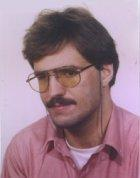
\includegraphics[width=0.7\textwidth]{sections/malte_slides/atof1}
            \end{subfigure}
            \begin{subfigure}[b]{0.45\textwidth}
                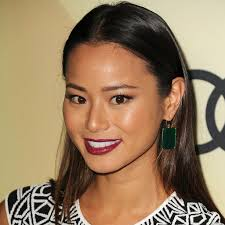
\includegraphics[width=1\textwidth]{sections/malte_slides/atof2}
            \end{subfigure}
            \begin{subfigure}[b]{0.6\textwidth}
                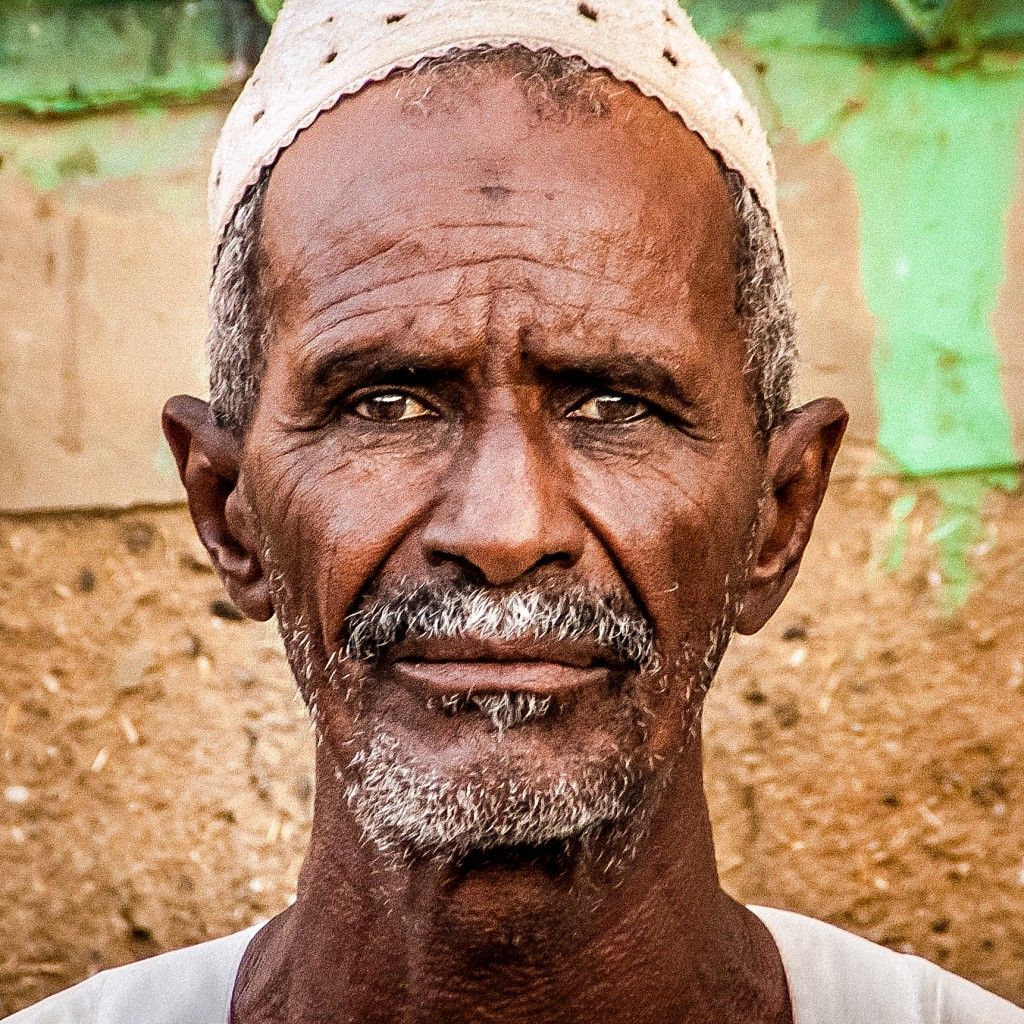
\includegraphics[width=0.95\textwidth]{sections/malte_slides/atof3}
            \end{subfigure}
        \end{figure}
    \end{columns}
\end{frame}

\begin{frame}{Results}{AToF - Finetuning layer 3}
    \begin{columns}
        \column{0.7\textwidth}
        \begin{figure}
            \centering
            \begin{subfigure}[b]{0.48\textwidth}
                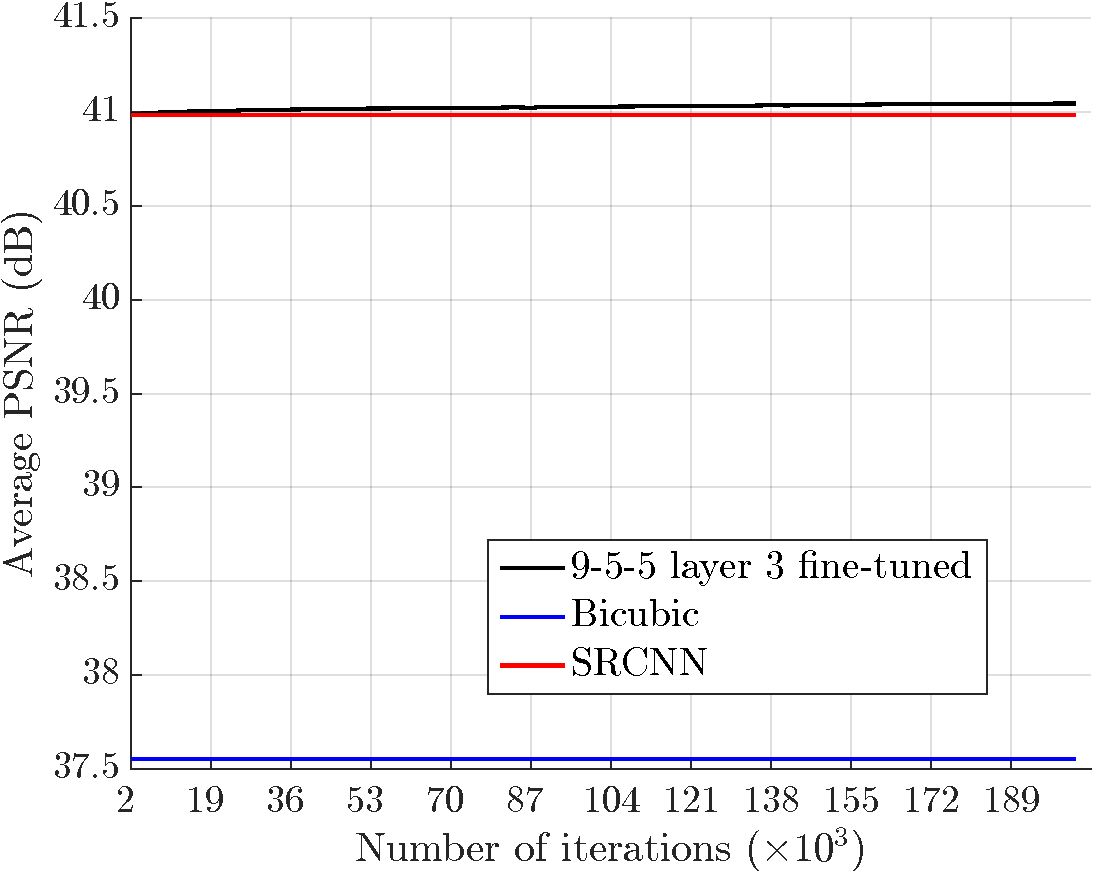
\includegraphics[width=\textwidth]{sections/malte_slides/atof-l3-results-aleix5.pdf}
                \vspace*{-2mm}
                \caption*{\scriptsize AR5}
            \end{subfigure}
            \begin{subfigure}[b]{0.48\textwidth}
                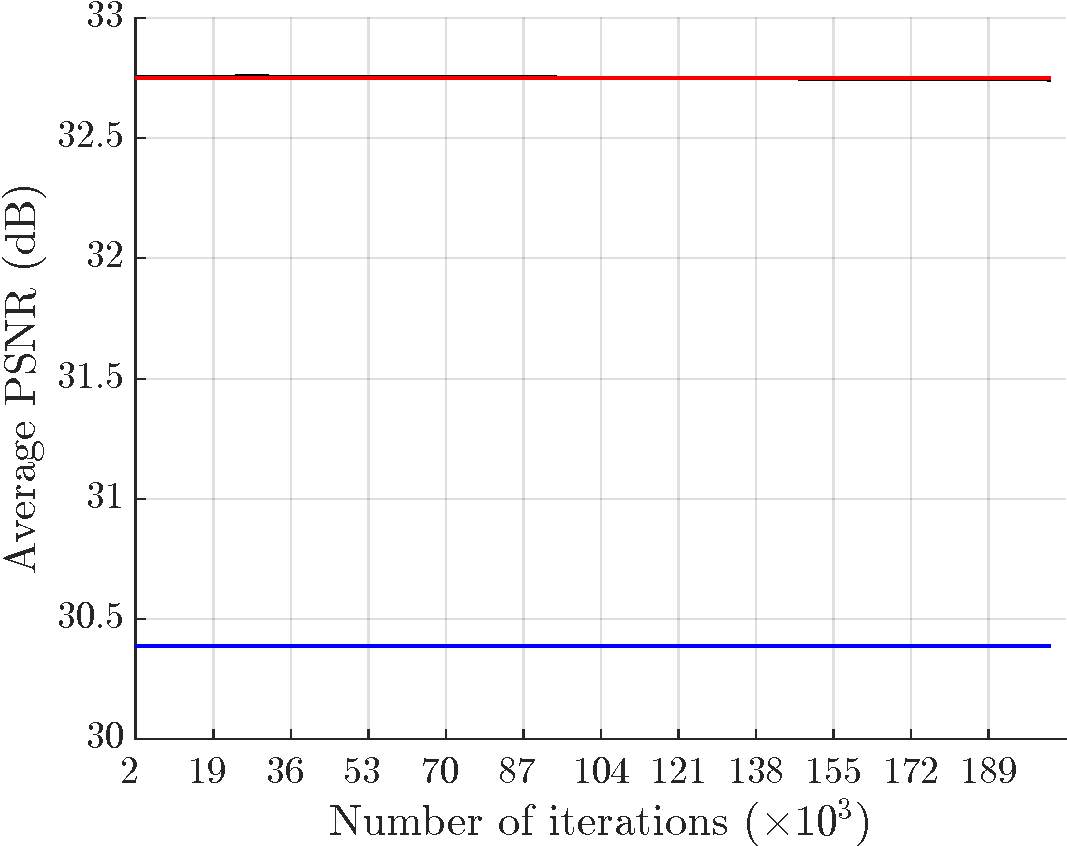
\includegraphics[width=\textwidth]{sections/malte_slides/atof-l3-results-set5.pdf}
                \vspace*{-2mm}
                \caption*{\scriptsize Set5}
            \end{subfigure}
            \begin{subfigure}[b]{0.48\textwidth}
                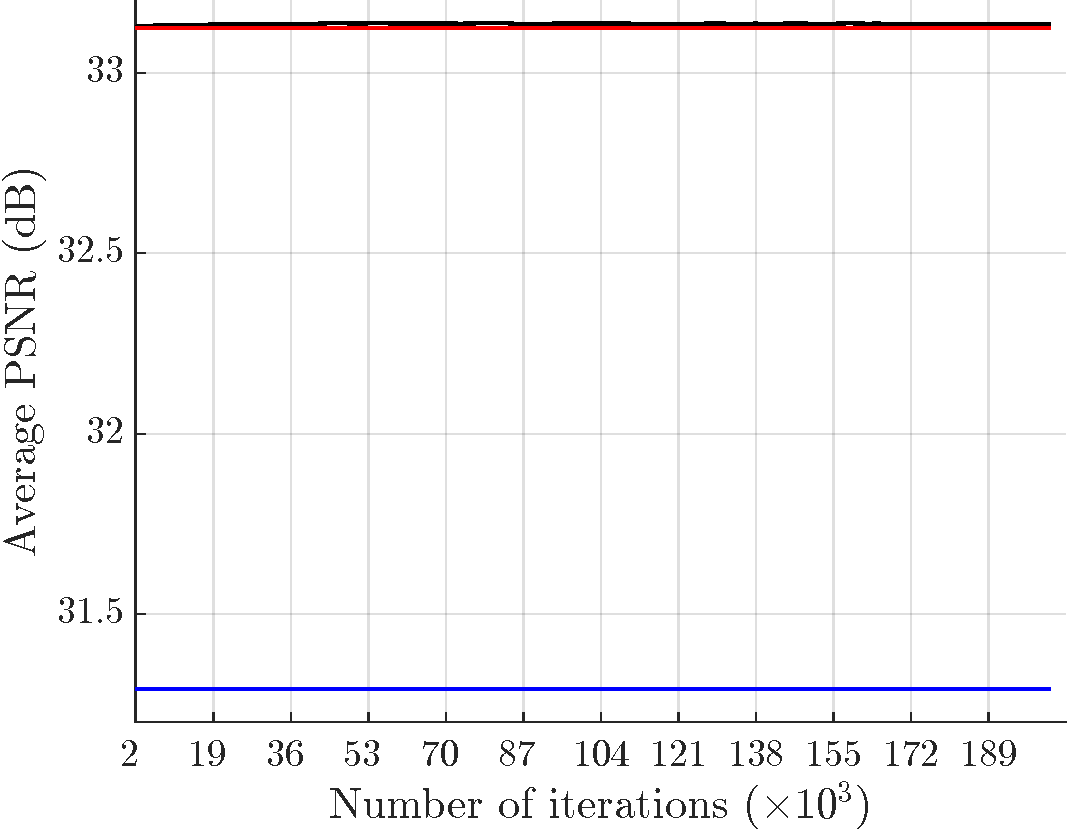
\includegraphics[width=\textwidth]{sections/malte_slides/atof-l3-results-tdrf.pdf}
                \vspace*{-2mm}
                \caption*{\scriptsize TDRF}
            \end{subfigure}
        \end{figure}

        \visible<2->{
        \column{0.3\textwidth}
        \begin{itemize}
            \item No significant difference
            \item No sign on further improvement
        \end{itemize}
    }
    \end{columns}
\end{frame}

\begin{frame}{Research}{Overview}
    \begin{figure}
        \centering
        \includegraphics[width=0.9\textwidth]{sections/malte_slides/step3.tex}
    \end{figure}
\end{frame}

\begin{frame}{Results}{AR500 - Finetuning layer 2 and 3}
    \begin{columns}
        \column{0.5\textwidth}
        \begin{block}{AR500}
            \begin{itemize}
                \item Same camera and setup.
                \item No variation in resolution.
                \item Minor variation in face size and background.
            \end{itemize}
        \end{block}
        \column{0.5\textwidth}
        \begin{figure}
            \centering
            \begin{subfigure}[b]{0.45\textwidth}
                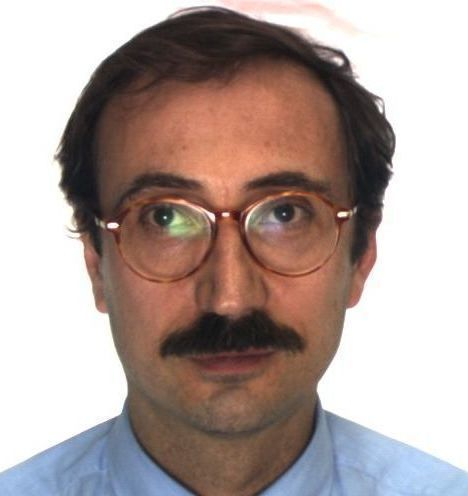
\includegraphics[width=\textwidth]{sections/malte_slides/ar1}
            \end{subfigure}
            \begin{subfigure}[b]{0.45\textwidth}
                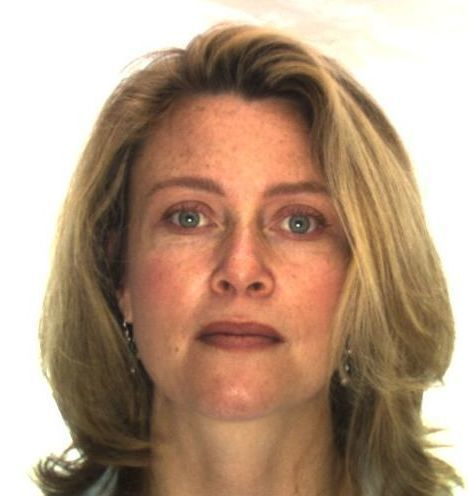
\includegraphics[width=\textwidth]{sections/malte_slides/ar2}
            \end{subfigure}
            \begin{subfigure}[b]{0.45\textwidth}
                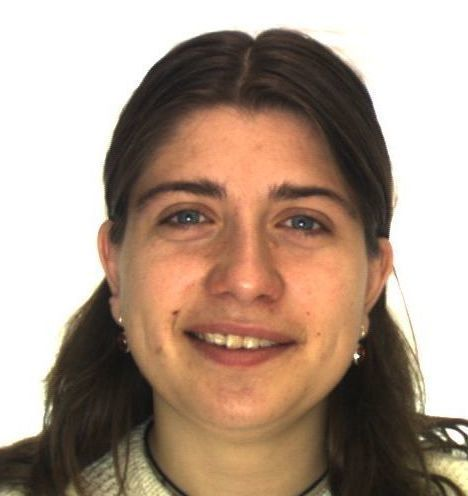
\includegraphics[width=\textwidth]{sections/malte_slides/ar3}
            \end{subfigure}
        \end{figure}
    \end{columns}
\end{frame}

\begin{frame}{Results}{AR500 - Finetuning}
    \begin{columns}
        \column{0.7\textwidth}
        \begin{figure}
            \centering
            \begin{subfigure}[b]{0.48\textwidth}
                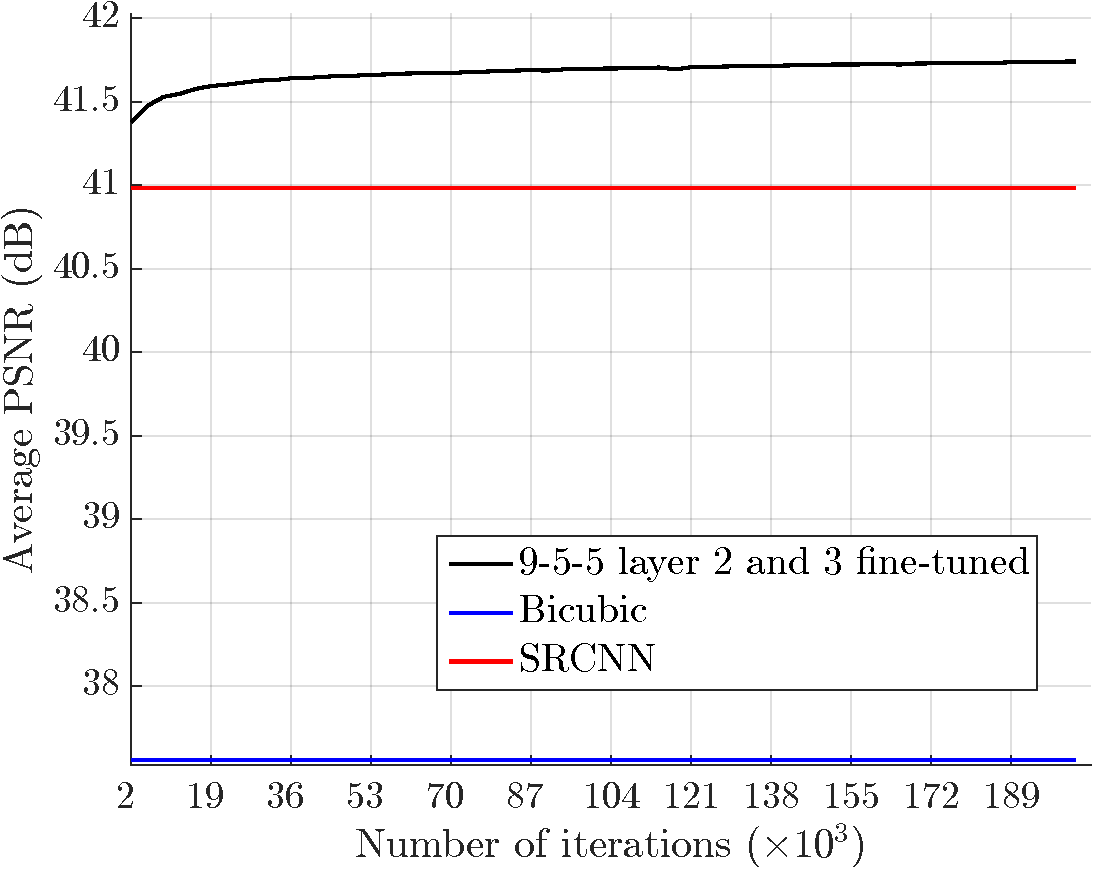
\includegraphics[width=\textwidth]{sections/malte_slides/fine23-results-aleix5.pdf}
                \vspace*{-2mm}
                \caption*{\scriptsize AR5}
            \end{subfigure}
            \begin{subfigure}[b]{0.48\textwidth}
                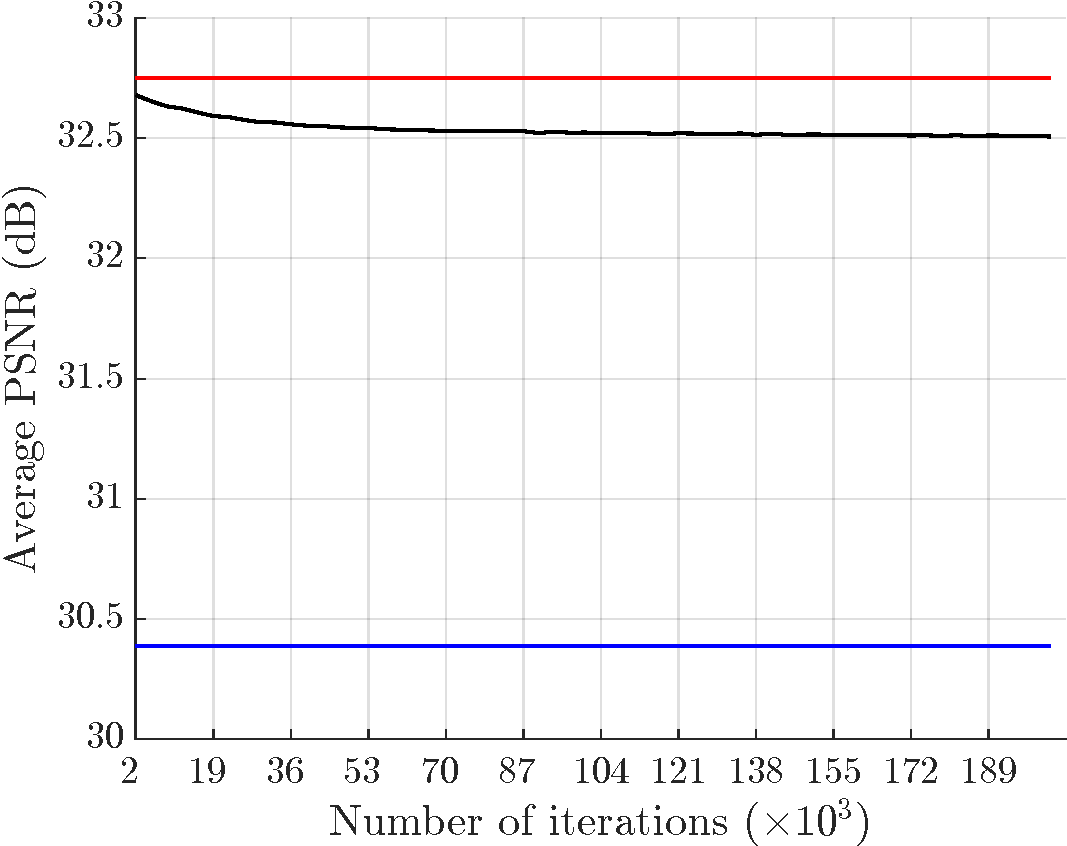
\includegraphics[width=\textwidth]{sections/malte_slides/fine23-results-set5.pdf}
                \vspace*{-2mm}
                \caption*{\scriptsize Set5}
            \end{subfigure}
            \begin{subfigure}[b]{0.48\textwidth}
                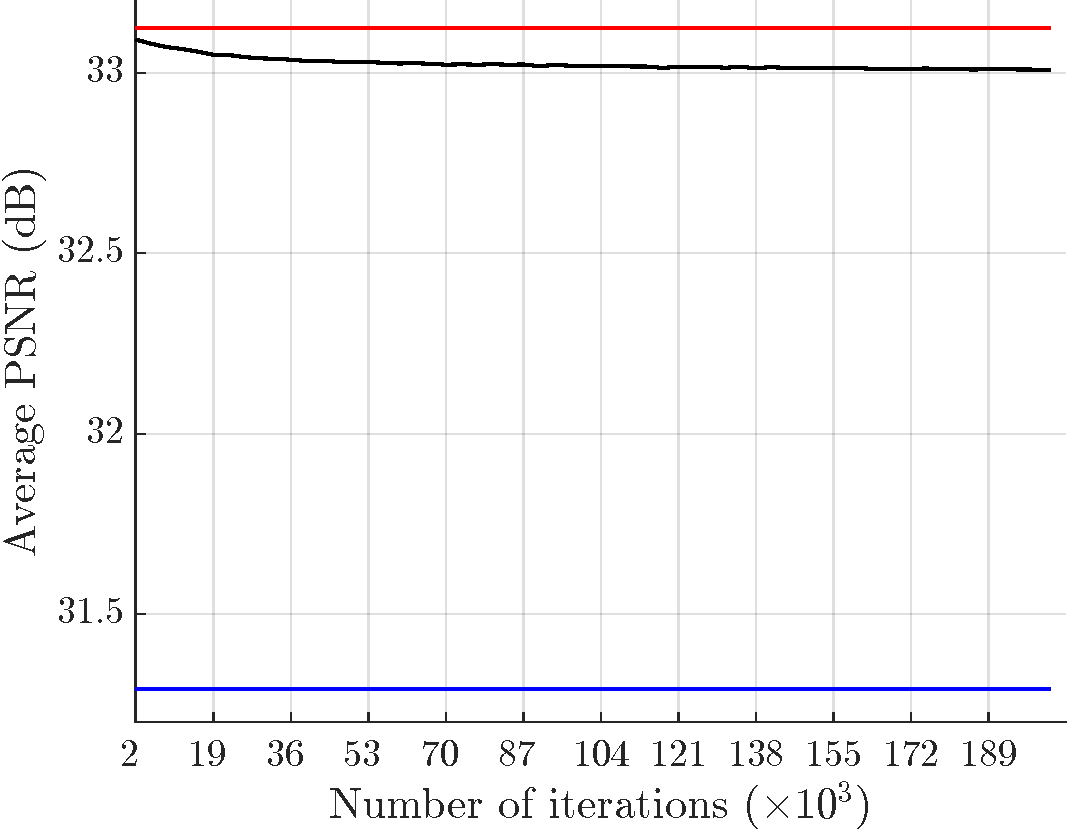
\includegraphics[width=\textwidth]{sections/malte_slides/fine23-results-tdrf.pdf}
                \vspace*{-2mm}
                \caption*{\scriptsize TDRF}
            \end{subfigure}
        \end{figure}

        \visible<2->{
        \column{0.45\textwidth}
        \begin{itemize}
            \item Worse on images from other environments
            \item Increase of \underline{0.75dB PSNR} on images from similar environments
            \item May show further improvements with more training
        \end{itemize}
    }
    \end{columns}
\end{frame}

\begin{frame}{Research}{Overview}
    \begin{figure}
        \centering
        \includegraphics[width=0.9\textwidth]{sections/malte_slides/step4.tex}
    \end{figure}
\end{frame}

\begin{frame}{Results}{AR500 - Retraining}
    \begin{columns}
        \column{0.7\textwidth}
        \begin{figure}
            \centering
            \begin{subfigure}[b]{0.48\textwidth}
                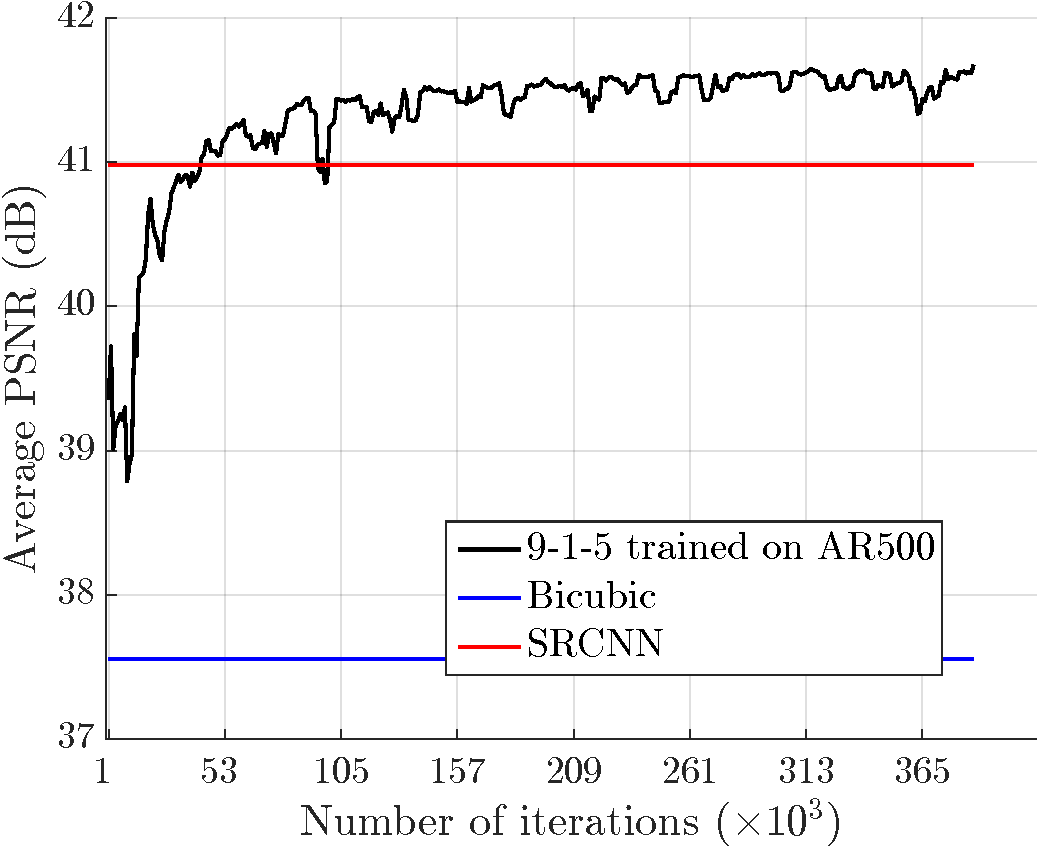
\includegraphics[width=\textwidth]{sections/malte_slides/915-results-aleix5.pdf}
                \vspace*{-2mm}
                \caption*{\scriptsize AR5}
            \end{subfigure}
            \begin{subfigure}[b]{0.48\textwidth}
                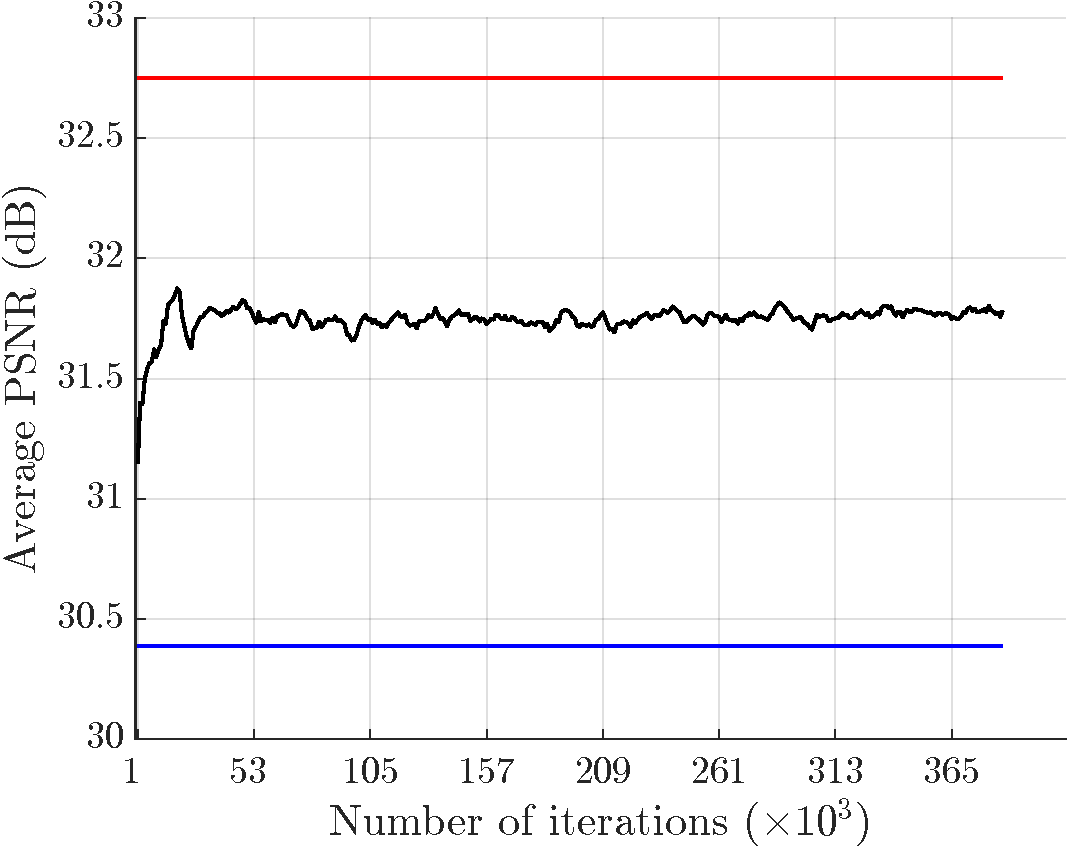
\includegraphics[width=\textwidth]{sections/malte_slides/915-results-set5.pdf}
                \vspace*{-2mm}
                \caption*{\scriptsize Set5}
            \end{subfigure}
            \begin{subfigure}[b]{0.48\textwidth}
                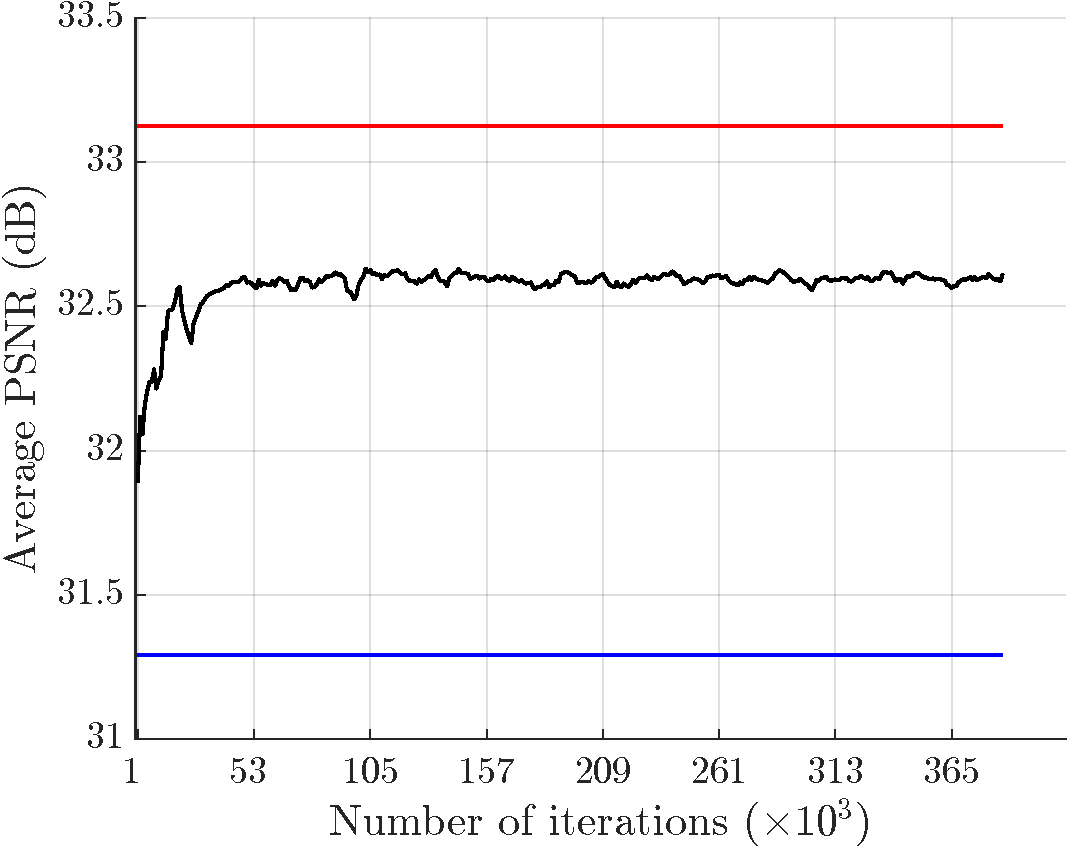
\includegraphics[width=\textwidth]{sections/malte_slides/915-results-TDRF.pdf}
                \vspace*{-2mm}
                \caption*{\scriptsize TDRF}
            \end{subfigure}
        \end{figure}

        \visible<2->{
        \column{0.4\textwidth}
        \begin{itemize}
            \item Long training time
            \item More or less same results as finetuning
        \end{itemize}
    }
    \end{columns}
\end{frame}

\begin{frame}{Large Face Dataset}{New results}
    \begin{block}{Impact of the dataset size in regard to finetuning?}
        \visible<2->{
            Full LFD training set (13.300 images):
        \begin{table}[h]
            \footnotesize
            \centering
            \begin{tabularx}{\textwidth}{|l|X|X|X|X|X|}
                \hline
                \textbf{Dataset} & \textbf{Bicubic} & \textbf{SRCNN}  &\textbf{SRCNN$_{AToF}^{2/3}$} & \textbf{SRCNN$_{LFD}^{2/3}$} \\ \hline
                AR5              & 37.5565/0.9735   & 40.9816/\textbf{0.9814}  & \textbf{41.1726}/0.9813             & 39.7784/0.9722 \\ \hline
                Set5             & 30.3900/0.8682   & 32.7500/\textbf{0.9090}  &   \textbf{32.7551}/0.9075           & 32.5721/0.9053 \\ \hline
                TDRF             & 31.2926/0.8706   & 33.1255/\textbf{0.9034}  &  \textbf{33.1364}/0.9029            & 33.0869/0.9026 \\ \hline
                LFD              & 32.1229/0.9085   & 34.1332/0.9338           &  34.2664/0.9342                     & \textbf{34.5168/0.9359} \\ \hline
            \end{tabularx}
        \end{table}
    } 
    \end{block}
    \visible<3->{
        \begin{columns}
            \column{0.5\textwidth}
        LFD-5\% training set (666 images):
        \begin{table}[h]
            \footnotesize
            \centering
            \begin{tabular}[c]{|l|l|}
                \hline
                \textbf{Dataset} & \textbf{SRCNN$_{LFD-5\%}^{2/3}$} \\ \hline
                AR5              & \underline{41.1401}/0.9813                   \\ \hline
                Set5             & 32.5356/0.9044                   \\ \hline
                TDRF             & 33.0602/0.9021                   \\ \hline
                LFD              & 34.4127/0.9339                   \\ \hline
            \end{tabular}
        \end{table}
        }\visible<4->{
    \column{0.5\textwidth}
    \begin{itemize}
        \item No significant change in performance
    \end{itemize}}
\end{columns}
\end{frame}

\section{Conclusion}
\begin{frame}{Conclusion}{}
    \begin{block}{Conclusion}
        \begin{itemize}
            \item It is possible to increase the PSNR performance on images from the same environment
            \item Minor visual difference on the images we have tested on
        \end{itemize}
    \end{block}
    \visible<2->{
        \begin{figure}
            \centering
            \begin{subfigure}[b]{0.235\textwidth}
                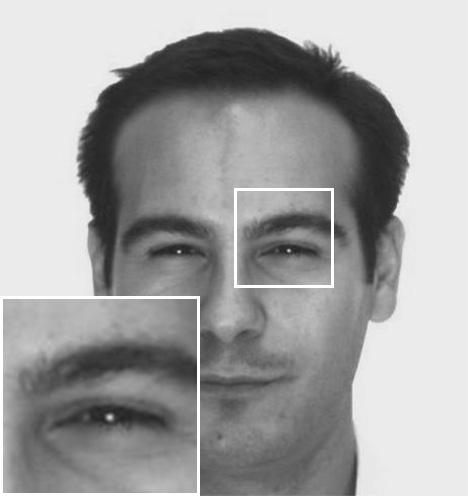
\includegraphics[width=\textwidth]{sections/malte_slides/915-gt.jpg}
                \caption*{\scriptsize Ground truth}
            \end{subfigure}
            \begin{subfigure}[b]{0.235\textwidth}
                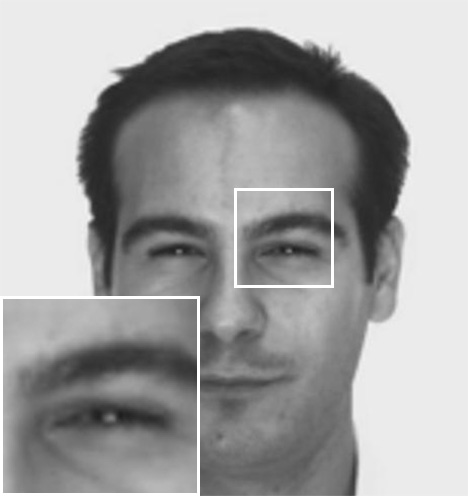
\includegraphics[width=\textwidth]{sections/malte_slides/915-bic.jpg}
                \caption*{\scriptsize Bicubic: 39.04}
            \end{subfigure}
            \begin{subfigure}[b]{0.235\textwidth}
                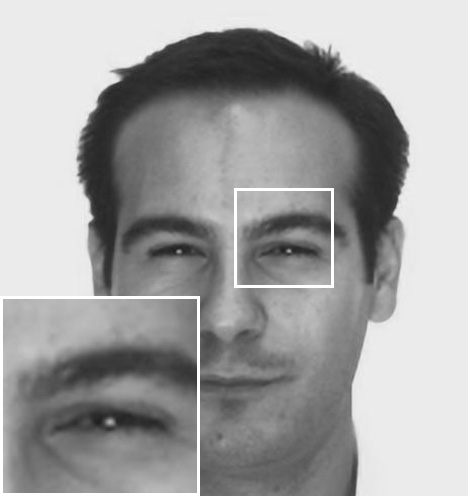
\includegraphics[width=\textwidth]{sections/malte_slides/srcnn955.jpg}
                \caption*{\scriptsize SRCNN 9-5-5: 42.49}
            \end{subfigure}
            \begin{subfigure}[b]{0.235\textwidth}
                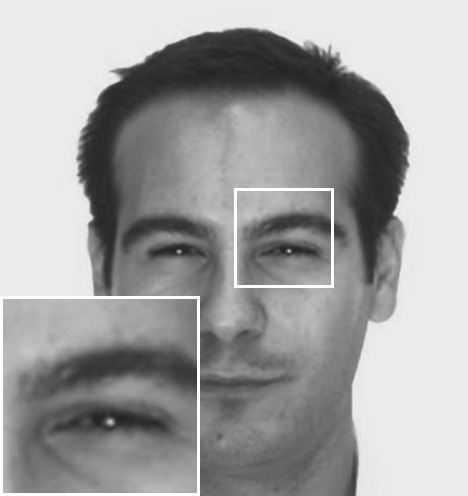
\includegraphics[width=\textwidth]{sections/malte_slides/arFine-finetune.jpg}
                \caption*{\scriptsize SRCNN$_{AR}^{2/3}$: 43.41}
            \end{subfigure}
        \end{figure}
    }
    \visible<3->{
    \begin{itemize}
        \item Difficult to improve performance on all types of face images in one system
    \end{itemize}
}
\end{frame}

\section{Future work}
\begin{frame}{Future work}{}
    \begin{block}{Future work}
        \begin{itemize}
            \item Datasets with images of faces only (no background) 
            \item Other image degradations beside downscaling
            \item Deeper architecture
            \item Direct investigation of improvements on surveillance images.
                \begin{itemize}
                    \item Train networks on specific cameras and environments
                \end{itemize}
        \end{itemize}
    \end{block}
\end{frame}

\begin{frame}{Future work}{Datasets}
    \begin{block}{Faces only}
        \begin{figure}
            \centering
            \begin{subfigure}[b]{0.15\textwidth}
                \centering
                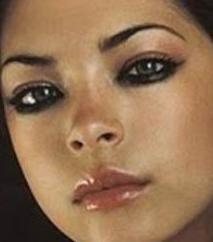
\includegraphics[width=\textwidth]{sections/malte_slides/crop5}
            \end{subfigure}
            \begin{subfigure}[b]{0.15\textwidth}
                \centering
                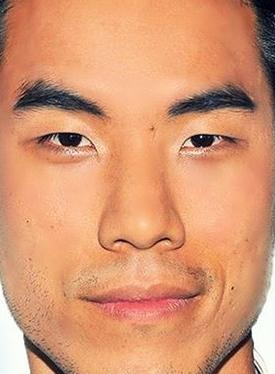
\includegraphics[width=\textwidth]{sections/malte_slides/crop2}
            \end{subfigure}
            \begin{subfigure}[b]{0.15\textwidth}
                \centering
                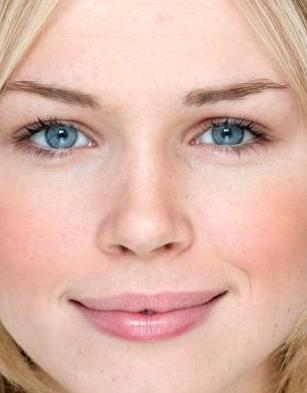
\includegraphics[width=\textwidth]{sections/malte_slides/crop6}
            \end{subfigure}
            \begin{subfigure}[b]{0.15\textwidth}
                \centering
                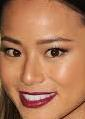
\includegraphics[width=\textwidth]{sections/malte_slides/crop4}
            \end{subfigure}
            \begin{subfigure}[b]{0.15\textwidth}
                \centering
                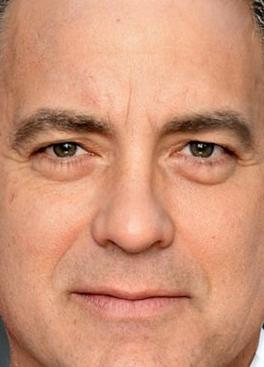
\includegraphics[width=\textwidth]{sections/malte_slides/crop1}
            \end{subfigure}
        \end{figure}
    \end{block}
    \visible<2->{
    \begin{block}{Degradations}
        \begin{itemize}
            \item Blur
            \item Noise
        \end{itemize}
    \end{block}
}
\end{frame}

\begin{frame}{Future work}{Architecture}
    \begin{block}{Deeper architecture}
        \begin{itemize}
            \item The research of Kim et al.\footnotemark ~ has shown improvements in performance for deeper networks
            \item Sophisticated training methods are needed
        \end{itemize}
    \end{block}
\footnotetext{J. Kim, J. K. Lee, and K. M. Lee, “Accurate Image Super-Resolution Using Very Deep Convolutional Networks,” ArXiv e-prints, Nov. 2015.}
\end{frame}

\begin{frame}[plain,noframenumbering] % the plain option removes the header from the title page
  \titlepage
\end{frame}


